\documentclass{book}


% Page size
\usepackage[a5paper]{geometry}


% Font
\usepackage{fontspec}
\setmainfont{Clara}


% Typesetting
\usepackage{microtype}


% Colors
\usepackage[dvipsnames]{xcolor}
\definecolor{darkgray}{gray}{0.35}


% Languages
\usepackage[english, latin]{babel}


% Figures
\usepackage{graphicx}


% Initials
\usepackage{lettrine}


% Columns
\usepackage{paracol}


% Line spacing
\usepackage{setspace}


% Paragraph spacing and indents
\setlength{\parskip}{0.75\baselineskip}
\setlength{\parindent}{0pt}


% Decorative borders
%\usepackage[object=vectorian]{pgfornament}
%\usepackage{tikz}


% Remove page numbers when using cleardoublepage
\usepackage{emptypage}


% Margin notes inside text columns
\usepackage{wrapfig}


% Math
\usepackage{amsmath}


% Put page number at bottom
\pagestyle{plain}



\begin{document}

\pagenumbering{roman} 

{\fontsize{11}{11} \selectfont

\begin{titlepage}
\begin{center}
{\bfseries \lsstyle
{\Large CRONICA}

\vspace{0cm}

{\color{BrickRed} \Huge JOCELINI \\ \vspace*{0.5cm} DE BRAKELONDA,}

\vspace{0.4cm}

{\Large DE REBUS GESTIS SAMSONIS}

\vspace{0.2cm}

{\Large ABBATIS MONASTERII}

\vspace{0.4cm}

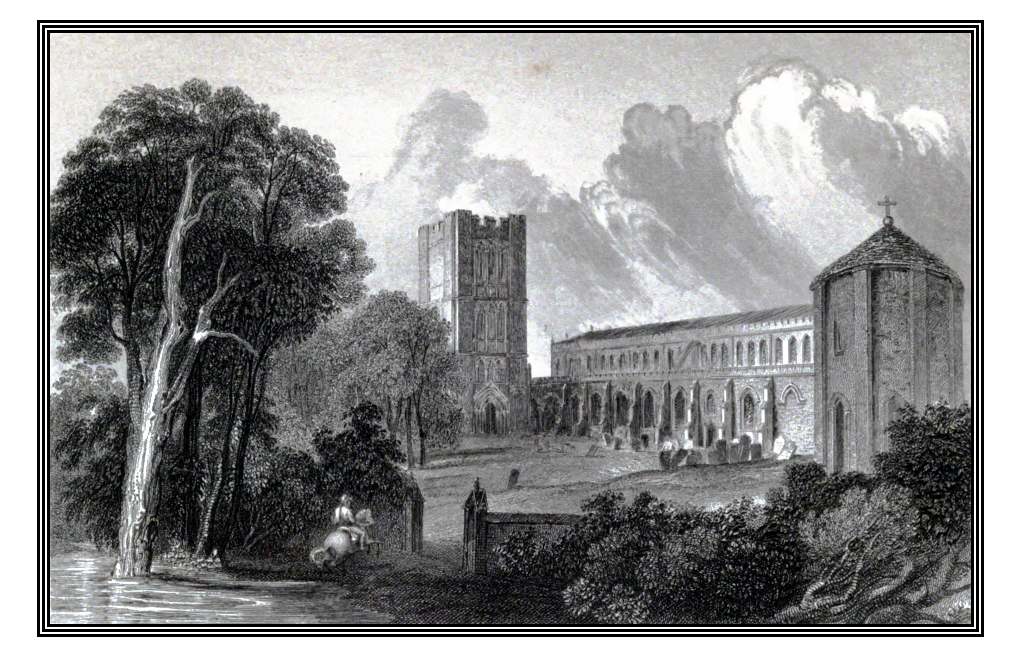
\includegraphics[scale=0.37]{fig/abbey.png}

\vspace{0.4cm}

{\color{BrickRed} \Huge SANCTI \AE{}DMUNDI.}

\vspace{0.2cm}

}
\end{center}
\end{titlepage}


\thispagestyle{empty}
\begin{center}

{\setlength{\parskip}{3mm}

Cronica de rebus gestis Samsonis abbatis
 
(Harl.\ MS.\ 1005 ff.\ 127r--170v)

Jocelin of Brakelond

\vspace*{5mm}

{\small \emph{Compiled, reset and reprinted \&c.}}

R.\ Creswell

Oxford

MMXXI

}

\end{center}

\vfill

{\setlength{\parskip}{1mm} \small

\emph{Frontispiece---}

G.\ F.\ Sargent and J.\ C.\ Varrall in \emph{The Book of Shakespeare Gems: In a Series of Landscape Illustrations of the Most Interesting Localities of Shakespeare's Dramas}, Bohn, London, \oldstylenums{1846}.

\vspace{0.4cm}

\emph{Latin text---}

Ed.\ T.\ Arnold: \emph{Memorials of St.\ Edmund's Abbey}, Vol.\ \oldstylenums{1}, Rerum Britannicarum Medii \AE{}vi Scriptores, The Lords Commissioners of Her Majesty's Treasury, Under the Direction of the Master of the Rolls, London, \oldstylenums{1890}.


\vspace{0.4cm}

\emph{English translation, introduction and footnotes---}

Trans.\ ed.\ L.\ C.\ Jane, intr.\ Abbot Gasquet: \emph{The Chronicle of Jocelin of Brakelond, Monk of St.\ Edmundsbury: A Picture of Monastic and Social Life in the XII{\tiny TH} Century}, Chatto \& Windus, London, \oldstylenums{1907}.

}


\newpage

\thispagestyle{empty}
\begin{center}

\hspace{0pt}
\vfill

{\setstretch{1.1}

\parbox{5.5cm}{
\makebox[0pt][r]{\emph{``}}{\emph{Fly, noble English, you are bought and sold;\\
Unthread the rude eye of rebellion\\
And welcome home again discarded faith.\\
Seek out King John and fall before his feet;\\
For if the French be lords of this loud day,\\
He means to recompense the pains you take\\
By cutting off your heads: thus hath he sworn\\
And I with him, and many moe with me,\\
Upon the altar at Saint Edmundsbury;\\
Even on that altar, where we swore to you\\
Dear amity and everlasting love.''}
}
}
}

\vfill
\hspace{0pt}

\end{center}

\cleardoublepage

\begin{center}


\hspace{0cm}\vspace{1.4cm}

\parbox{8cm}{
{\scshape
A veritable monk of Bury St.\ Edmunds is worth attending to, if by chance made visible and audible. Here he is; and in his hand a magical speculum, much gone to rust, indeed, yet in fragments still clear; wherein the marvellous image of his existence does still shadow itself, though f\vphantom iitfully, and as with an intermittent light.\\
}

\hspace{0pt}\hfill Carlyle --- \emph{Past and Present}.
}

\end{center}

\vspace{1cm}

{\setstretch{1.05}

\lettrine[lines=4]{\color{BrickRed}F}{ew} medi\ae{}val documents have exercised a greater fascination over men's minds in these latter days than ``The Chronicle of Jocelin of Brakelond.'' More than sixty years ago the publication of the Latin text of this history, by the Camden Society, attracted the attention of the great Thomas Carlyle, and furnished him with material for sketching his picture of ``The Ancient Monk,'' which occupied the entire second book of his \emph{Past and Present}. Although the modern sage in his own rugged way affected no little contempt for what he called this ``extremely foreign book,'' and for ``the monk-Latin'' in which it was written, it is evident that Jocelin's simple story of the wise, firm, yet withal gentle rule ofa medi\ae{}val abbot over a great English monastery cast a spell over him, the influence of which can be detected in every page of his delightful and almost surprisingly sympathetic account of Abbot Samson and of Edmundsbury.

In this case the \emph{Past}, as Carlyle read it in the ``Chronicle,'' was so entirely different from the \emph{Present}, as he knew it in his day, that the wonder is not that he was fascinated by it, but that he was able with its help to paint so true and living a picture and to fashion so fitting a frame in which to set it. For to him, without doubt, the story dealt with what he regarded as ``vanished existences''---``ideas, life-furniture, whole workings and ways,'' which were not only \emph{Past}, but gone beyond recall, and ``covered deeper than Pompeii with the lava-ashes and inarticulate wreck of seven hundred years!''

And indeed it cannot be denied that the ideals and aspirations, as revealed to us in the history of Abbot Samson and, so far as we know, in the life story of his biographer Jocelin, are of a higher and almost a different order to those of our modern world. To men of their calling in those far-off times, the natural and the supernatural were united and intermingled in the simplest and most ordinary way. Their very notions of the unseen world are almost sufficient to take away the breath of those whose lots have been cast in this more material and prosaic age of doubts and disbeliefs. To Samson, and Jocelin, and their fellow-monks at Edmundsbury in the twelfth century, heaven, as a great writer has said of earlier English monasticism, was hardly even ``next door.'' The future life was merely the present continued, and each man went forth to his task as it came and laboured at it day by day, not with any idea of finishing it, but only of carrying on for the span of his allotted existence. They built, and planted, and wrote till the end came, and then they went to heaven and others stepped into their places and took up the common work. It was indeed a ``simple life:'' it was almost Arcadian in its picturesque simplicity, and, as Cardinal Newman says of the same life in the days of our Venerable Bede, it reminds us of those times in the dayspring of the world, when Adam delved and Abel watched the flocks, and Noah tended his vines, and angels visited them.

This living belief in the nearness and all-importance of the supernatural is the key-note of Jocelin's charming story of a few brief years in the long history of an old English abbey, a new translation of which is here given to the public. As a story, however, Brakelond's ``Chronicle'' is not wholly, nor indeed mostly, either mysterious or incredible: there are troubles, and trials, and difficulties enough recounted by the writer; and at every turn we may see evidences of human nature and even of human struggles and passions, which are sufficient, and as some may perhaps think, more than sufficient, to show us that it is a history of men, and not of angels, which the old monk is setting forth so naturally and so truthfully. At any rate, there is quite sufficient of the human element in the narrative to give most of us a human interest in the story.

And this itself is proof that Jocelin is a true chronicler of what really took place, and no mere romancer tempted to edit or suppress entirely what might not be unto ``edification.'' He manifests no desire to make himself or his brethren appear other than what they were in reality---that is, thorough Englishmen, with strong wills and human passions, which, though these same passions might occasionally appear to gain the mastery, they were at all times endeavouring to subdue unto God's service by the help of His grace and through the broad-minded provisions of St.\ Benedict's Rule. The actors who appear in this living drama, though they are for the most part monks, are obviously men, natural and human enough in all their works and words; but these men are at the same time also monks, endeavouring to raise their minds and hearts to supernatural ideals, and striving to attain to that personal communion with God which is the aim and object of all true religion and of all religious observance and practice. This is ``another world truly,'' writes Carlyle, ``and this present poor distressed world might get some profit by looking wisely into it, instead of foolishly. But at lowest, O dilettante friend, let us know always that it \emph{was} a world, and not a void infinite of grey haze with phantasms swimming in it. These old St.\ Edmundsbury walls, I say, were not peopled with phantasms, but with men of flesh and blood, made altogether as we are. Had thou and I then been, who knows but we ourselves had taken refuge from an evil Time and fled to dwell here, and meditate on an Eternity, in such fashion as we could? Alas, how like an old osseous fragment, a broken blackened shinbone of the old dead Ages, this black ruin looks out, not yet covered by the soil; still indicating what a once gigantic Life lies buried there! It is dead now, and dumb; but was alive once and spake. For twenty generations, here was the earthly arena where painful living men worked out their life-wrestle,---looked at by Earth, by Heaven and Hell. Bells tolled to prayers; and men of many humours, various thoughts, chanted Vespers and Matins;---and round the little islet of their life rolled for ever (as round ours still rolls, though we are blind and deaf) the illimitable Ocean, tinting all things with \emph{its} eternal hues and reflexes, making strange prophetic music! How silent now!''

\textbf{The Author.}---Jocelin de Brakelond, the writer of the Chronicle called by his name, was a monk of Edmundsbury. The date of his birth is uncertain, but as he became a novice in that abbey in \oldstylenums{1173}, we may suppose that he was born not later than \oldstylenums{1156}. It has been conjectured that he was a native of Bury St.\ Edmunds, and that his name Brakelond was derived from that of an ancient street of the city, in accordance with the common practice of calling monks by the name of the place from which they came to religion. Little more is known about him than he tells us incidentally in the course of his narrative, but one of his contemporaries in the monastery speaks of him as ``a man of excellent religious observance, as well as a power both in word and work''---\emph{eximiae religionis, potens sermone et opere}. Carlyle sees him in his writing as a man of a ``patient, peaceable, loving, clear-smiling nature.'' A ``wise simplicity,'' he adds, ``is in him; much natural sense; a veracity that goes deeper than words.'' What more can we desire in a writer, especially when we may add that he shows himself to have been a cultured man, acquainted with the ancient authors, quoting Virgil and Horace and Ovid? His knowledge of the Bible is naturally extensive, and, as was common in those days, his very phraseology is obviously founded upon the sacred text. He once likewise cites, with acknowledgment, a short passage from the more modern Ralph de Diceto's \emph{Imagines Historiarum}. Our latter-day philosopher praises him also because he shows himself to have ``a pleasant wit; and to love a timely joke, though in a mild subdued manner; very amiable to see.''

In \textsc{a.d.} \oldstylenums{1173}, as just noted, Jocelin entered the community and passed under the care of Samson of Tottington, who subsequently became abbot, but who was then Master of novices. The then abbot, Hugh, was old, and although a high standard of the religious exercises and of the monastic life inside the cloister was maintained, the temporalities were in a sad state, and year by year tended to get from bad to worse, so that Jocelin's early experiences of monastic life were connected with anxieties about the load of debt to money-lenders under which Edmundsbury groaned.

He tells us that he had himself seen bonds for repayment made out to the Jews, under which, for failure to meet the sums falling due, the original loan had grown in eight years from £\oldstylenums{100} to £\oldstylenums{800}. No wonder that the youthful religious questioned his Master of novices as to why some remedy was not found by those in authority for a state of things which meant temporal ruin and disgrace for the community of Edmundsbury.

In \oldstylenums{1180} Abbot Hugh met with an accident and died. After a period of a year and three months the former Master of novices, Samson, then the provident Sacrist, was chosen in his place. It was during this period of vacancy that, in recording something which happened in the monastery, Jocelin incidentally makes mention of another literary work of his own, namely, the \emph{Book of the Miracles of St.\ Robert}, a boy supposed to have been martyred by the Jews in \oldstylenums{1181}, who was entombed in the church at Edmundsbury.

On the election of Samson, Jocelin was appointed his chaplain, and this brought him into the closest connection with the abbot for six years. In \oldstylenums{1198} and \oldstylenums{1200} he was Guest-master, and in \oldstylenums{1212} he held the office of Almoner. In all these offices the future chronicler had exceptional means of acquiring information, and these he utilised in writing the story of Abbot Samson's administration, which is introduced by a vivid sketch of the temporal disorder of the house in the closing years of Abbot Hugh. His Chronicle covers the period of the history of Edmundsbury from \oldstylenums{1173} to \oldstylenums{1190}, and, as he says in the beginning, ``he took care to write only what he himself saw and heard.'' The date of his death is uncertain.

\textbf{The ``Chronicle.''}---The Latin text of \emph{Cronica Joceline} is found complete only in one manuscript---Harl.\ MS.\ \oldstylenums{1005}---in the British Museum. It was printed for the first time by the Camden Society in \oldstylenums{1840} under the editorship of I.\ G.\ Gage Rokewood, who supplied a valuable Introduction and notes, of which subsequent editors have availed themselves. The text was likewise printed in Mr.\ Thomas Arnold's \emph{Memorials of St. Edmund's Abbey} (Rolls Series) I., pp. \oldstylenums{209}--\oldstylenums{336}.

In \oldstylenums{1844}, under the title \emph{Monastic and Social Life in the Twelfth Century, as exemplified in the Chronicle of Jocelin of Brakelond, A.D. \oldstylenums{1173}--\oldstylenums{1202}}, the work was translated by Thomas Edlyne Tomlins. Carlyle's work, \emph{Past and Present}, published in \oldstylenums{1843} had already drawn attention to the ``Chronicle of Jocelin,'' and another edition of Mr. Tomlins' work was called for in \oldstylenums{1849}. This translation has since appeared at least once, but for the present edition a new English version has been carefully prepared from the original Latin text of the Chronicle.

\emph{Abbot Samson.}---The central figure and, as we may say, ``the hero'' of Jocelin's story is, of course, Abbot Samson. He was born in \oldstylenums{1135} at Tottington, near Thetford, in Norfolk. His father appears to have died when Samson was young, and a pretty legend of a boyish dream in which St.\ Edmund extended his protection to the child against the assaults of the devil, and the recognition of the place seen in the dream as the gate of the monastery of St.\ Edmundsbury, when his mother had taken him with her on a pilgrimage to the shrine of the saint, led to his taking refuge in the cloister. He had received his early instruction from a schoolmaster named William of Diss, and he attained the degree of Master of Arts in the University of Paris. In this place we are not concerned with the events of his life: these may be read for the most part in the Chronicle of Jocelin of Brakelond. What alone seems to be called for in this brief Introduction is some account of his person and character as it is manifested in the scattered evidences of his acts.

If we want a picture of the man let us take Carlyle's, who sketches ``the substantial figure of a man with eminent nose, bushy brows, and clear-flashing eyes, his russet beard growing daily greyer,'' and his hair which, before his elevation to the abbot's chair, had been black, becoming daily more and more silvered with his many cares. We know something of the task that was before him when he gathered up the reins of office, and we may be sure he knew more. But as we see him in the pages of Jocelin, he was not the man to flinch from his duty, or to seek to let difficulties mend themselves by pretending that he did not see them. From the time that he walked barefooted into his church to be installed in the abbatial chair, he let all see that he was abbot and had come to rule. He had set his whole strength to accomplish a great task and his shoulders to sustain an almost overwhelming burden, when in the hour of his election he walked to the altar singing the \emph{Miserere mei} with his brethren. ``His head was held erect,'' says the faithful Jocelin, ``and his face showed no change,'' a portent which called from the king the remark: ``This abbot-elect seems to think himself capable of governing an abbey.''

``It is beautiful''---writes Carlyle in a philosophical appreciation of the principles of monastic government---``it is beautiful how the chrysalis governing-soul, shaking off its dusty slough and prison, starts forth winged, a true royal soul! Our new abbot has a right honest, unconscious feeling, without insolence as without fear or flutter, of what he is and what others are. A courage to quell the proudest, an honest pity to encourage the humblest. Withal there is a noble reticence in this Lord Abbot: much vain unreason he hears; lays up without response. He is not there to expect reason and nobleness of others, he is there to give them of his own reason and nobleness. Is he not their servant, who can suffer from them and for them; bear the burden their poor spindle-limbs totter and stagger under; and in virtue of \emph{being} their servant, govern them, lead them out of weakness to strength, out of defeat into victory?''

Abbot Samson ruled over his house for thirty years, and when in \oldstylenums{1212}, ten years after the end of Jocelin's Chronicle, he died, he was followed to the grave by a sorrowing community whose unstinted reverence and affection he had won. An unknown monk of Edmundsbury, the author of another Chronicle of the house, thus wrote of him: ``On the \oldstylenums{30}th December, at St.\ Edmund's, died Samson, of pious memory, the venerable abbot of that place; after he had prosperously ruled the abbey committed to him for thirty years and had freed it from a load of debt, had enriched it with privileges, liberties, possessions and spacious buildings and had restored the worship of the church both internally and externally, in the most ample manner. Then bidding his last farewell to his sons, by whom the blessed man deserved to be blest for evermore, whilst they were all standing by and gazing with awe at a death which was a cause for admiration, not for regret, in the fourth year of the interdict he rested in peace."

The first business to which Abbot Samson applied himself after his election was the task of understanding and grappling with the deplorable financial state of his house. He insisted upon the immediate production of every claim against the monastery, and by personally visiting each of its many manors he gained a correct knowledge of its resources. Within twelve months he had formed his plans and had quieted every creditor: within twelve years the entire debt had been paid off, and he could turn his attention to building and adorning the house of St.\ Edmund. It is impossible to read the pages of Jocelin without seeing that the ruling idea of the abbot's life was his devotion to his great patron, St.\ Edmund. He was the servant, after God, of the saint, his representative and the upholder of his honour and privileges, the champion of his rights, the guardian of his property. Inspired by this thought he worked to make Edmundsbury worthy of its patron, and in his success he saw the result of the saint's intercession and protection.

``Apart from this special devotion to St.\ Edmund, it is easy to see,'' writes Mr.\ Thomas Arnold, ``that Samson was an earnestly religious man, and not a Christian by halves. After the news had come of the capture of Jerusalem by the Saracens, Samson took the loss of the Holy Places so much to heart, that from that time he wore undergarments of hair-cloth and abstained from the use of meat.''

He was, too, a thorough Englishman, and read admirably---\emph{elegantissime} - the Bible in English---\emph{scripturam anglice scriptam}---and ``he was wont to preach to the people in English---but in the dialect of Norfolk where he had been born and bred.'' On one occasion he gives as a reason, and as some may think, a somewhat strange reason, for appointing a monk to an office, that ``he did not know French.'' He was no doubt anxious to secure that St.\ Edmundsbury should be truly national, with its roots deep in the soil of his country, to teach it to build up its own traditions, and to let people see that it was a great \emph{English} house.

But Samson's work was not accomplished without grave anxiety, none the less because it was unseen by others. Though he walked upright with a smiling face, and had ever the courage to battle for the rights of his house when there was need, in a way that might make people regard him as a man of iron nerve possessed of a soul that never felt any trouble, nevertheless in the first fourteen years of his administration his black hair was blanched as white as snow, and Jocelin speaks of hearing his beloved master walking about when all were in bed and relieving his pent-up feelings with sighs and groans. Once the chronicler took courage to tell his master that he had thus heard him in his night vigil, and to this the abbot replied: ``'Tis no wonder: you (as my chaplain) share in the streets of my office, in the meat and drink, in the journeys and the like, but you little think what I have to do to provide for my house and family, or of the many and difficult matters of my pastoral office, which are always pressing upon me: these are the things which make my soul anxious and cause me to sigh.''

And so when Abbot Samson came to die, the thin veil which to him and his monks of Edmundsbury alone hid the world to come from their vision was parted, and the supernatural life eternal was revealed to him in the most natural of ways. He passed from labour for God and St.\ Edmundsbury, to rest in God and with his loved patron, carrying with him the full sheaves of his good works. Carlyle has only partially caught the idea when he writes: ``Genuine work alone, what thou workest faithfully, that is eternal.'' ``Yes,'' he concludes, ``a noble Abbot Samson resigns himself to oblivion; feels it no hardship, but a comfort; counts it as a still resting-place, for much sick fret, and fever, and stupidity, which in the night-watches often made his strong heart sigh.''
}
}


\begin{flushright}
\parbox{6cm}{
\begin{center}
\textsc{Francis Aidan Gasquet},\\
\vspace{0.1cm}
\emph{Abbot-President of the English Benedictines}.
\end{center}
}
\end{flushright}

\cleardoublepage
\footnotelayout{m}
\emergencystretch 1em
\pagenumbering{arabic} 




\begin{paracol}{2}

\lettrine[lines=4]{\color{BrickRed}Q}{uod} \begin{otherlanguage}{latin}vidi et audivi scribere curavi, qu\ae{}dam mala interserens ad cautelam, qu\ae{}dam bona ad usum,\linebreak qu\ae{}~\hspace{1.6cm}contigerunt in ecclesia sancti \AE{}dmundi in diebus nostris, ab anno quo Flandrenses capti sunt extra villam, quo habitum religionis suscepi, quo anno Hugo prior depositus est, et R.\ prior substitutus. 
\end{otherlanguage}

\switchcolumn

\lettrine[lines=4]{\color{BrickRed}I}{ have} undertaken to write of those things which I have seen and heard, and which have occurred in the church of Saint Edmund, from the year in which the Flemings were taken\footnote{The allusion is to the battle of Fornham, November, \oldstylenums{1173}. In this year the quarrel between Henry II. and his sons, culminated in a general rising both in Normandy and in England. Of the leaders of the rebellion in England, Robert de Bellemont, earl of Leicester, was the chief. Having gathered a force of mercenaries in the Low Countries, he landed at Walton, which he failed to take. After joining hands with Hugh Bigod, earl of Norfolk, at Framingham, and capturing Haughley, he attempted to force his way to his own estates. Meanwhile, the justiciar Richard de Lucy and Humphrey Bohun hastened south from their campaign against the Scots, and having been reinforced by the local levies, they succeeded in intercepting Leicester at Fornham St.\ Geneveve, on the river Lark, four miles south from Bury St.\ Edmund's. The rebels were easily defeated, and Leicester taken prisoner; of his mercenaries only a few escaped. An account of the battle, not very accurate, from the point of view of the St.\ Edmund's monks, is to be found in Appendix E of the first volume of the \emph{Memorials of St.\ Edmund's Abbey}, (Rolls Series). The escape of those mercenaries who did escape is attributed to the intervention of St.\ Edmund and St.\ Thomas.} without the town, in which year also I assumed the religious habit, and in which Prior Hugh was deposed and Robert made Prior in his room. And I have related the evil as a warning, and the good for an example.

\switchcolumn*

\begin{otherlanguage}{latin}
\begin{wrapfigure}[4]{l}{2.75cm}
\centering
\vspace{-0.1cm}
\parbox{2.75cm}{\footnotesize \color{BrickRed} \emph{How Abbot Hugh ruled the Church of St.\ Edmund.}\\ \centering \textsc{a.d.} \oldstylenums{1173}.}
\end{wrapfigure}
Tunc temporis senuit Hugo abbas, et aliquantulum caligaverunt ocuii ejus; homo pius et benignus, monachus religiosus et bonus, sed nec bonus nec providus in s\ae{}cularibus exercitiis: qui nimis confidebat suis et nimis eis credebat, de alieno potius quam de proprio pendens consilio. Ordo quidem et religio fervebant in claustro, et ea qu\ae{} ad ordinem spectant; sed exteriora male tractabantur, dum quisque, serviens sub domino simplice et jam senescente, fecit quod voluit, non quod decuit. Dabantur vill\ae{} abbatis et omnes hundredi ad firmam; nemora destruebantur; domus maneriorum minabantur ruinam; omnia de die in diem in deteriorem statum vertebantur. Unicum erat refugium et consolationis remedium abbati, denarios appruntare; ut saltem sic honorem domus su\ae{} posset sustentare. Non erat terminus Pasch\ae{} nec sancti Michaelis octo annis ante obitum ejus, quin centum libr\ae{} vel ducent\ae{} ad minus crescerent in debitum; semper renovabantur cart\ae{}, et usura qu\ae{} excrevit vertebatur in katallum.
 
\end{otherlanguage}

\switchcolumn

In those days Abbot Hugh\footnote{Hugh, prior of Westminster, was elected abbot in \oldstylenums{1157}, in succession to abbot Ording. According to Gervase (I., 163), he received his benediction from Theobald, archbishop of Canterbury, to whom he made profession of canonical obedience. According to the \emph{Chronica Buriensis} (\emph{Mem}.\ III., \oldstylenums{6}) he as confirmed by the bishop of Winchester. In any case, abbot Hugh, as it related in the text of the \emph{Chronicle of Jocelin} (p.\ \oldstylenums{6}), was freed from all obedience by pope Alexander III.} grew old, and his eyes were dim.\footnote{Gen.\ xxvii., \oldstylenums{1}.} He was a good and kindly man, a godfearing and pious monk, but in temporal matters he was unskilful and improvident. He relied too much on his own intimates and believed too readily in them, rather trusting to a stranger's advice than using his own judgment. It is true that discipline and the service of God, and all that pertained to the rule, flourished greatly within the cloister, but without the walls all-things were mismanaged. For every man, seeing that he served a simple and ageing lord, did not that which was right, but that which was pleasing in his own eyes. The townships and all the hundreds of the abbot were given to firm; the woods were destroyed, and the houses on the manors were on the verge of ruin; from day to day all things grew worse. The abbot's sole resource and means of relief was in borrowing money, that so it might at least be possible to maintain the dignity of his house. For eight years before his death, there was never an Easter or Michaelmas which did not see at least one or two hundred pounds added to the debt. The bonds were ever renewed, and the growing interest was converted into principal.

\switchcolumn*

\begin{otherlanguage}{latin}
Descendebat h\ae{}c infirmitas a capite in membra, a pr\ae{}lato in subjectos. Unde contigit quod quilibet obedientiarius haberet sigillum proprium, et debito se obligaret tam Judeis quam Christianis pro voluntate sua. S\ae{}pe capp\ae{} seric\ae{}, et ampull\ae{} aure\ae{}, et alia ornamenta ecclesi\ae{} impignorabantur, inconsulto conventu. Vidi cartam fieri Willelmo filio Isabel mille librarum et xl.; sed nec causam nec originem scivi. Vidi et aliam cartam fieri Isaac, filio Raby Joce, cccc.\ librarum, sed nescio quare. Vidi et tertiam cartam fieri Benedicto Judeo de Norwico, octies c.\ librarum et quater viginti; et h\ae{}c fuit origo et causa hujus debiti.
\end{otherlanguage}

\switchcolumn

This disease spread from the head to the members, from the ruler to his subjects. So it came to pass that if any official had a seal of his own, he also bound himself in debt as he listed, both to Jews and Christians. Silken caps, and golden vessels, and the other ornaments of the church, were often placed in pledge\footnote{This was illegal. Rokewode (\emph{Chron.\ Joc}., pp.\ \oldstylenums{106}--\oldstylenums{7}) gives instances of fines inflicted on Jews for taking church property in pawn, from the Pipe Rolls of Norfolk and Suffolk.} without the assent of the monastery. I have seen a bond made to William Fitzlsabel for a thousand and two score pounds, but know not the why nor wherefore. And I have seen another bond to Isaac, son of Rabbi Joce, for four hundred pounds, but know not wherefore it was made. I have seen also a third bond to Benedict, the Jew of Norwich, for eight hundred and fourscore pounds, and this was the origin and cause of that debt.

\switchcolumn*

\begin{otherlanguage}{latin}
Destructa fuit camera nostra, et recepit eam Willelmus sacrista volens vel nolens, ut eam instauraret; et occulte appruntavit a Benedicto Judeo xl.\ marcas ad usuram, et ei fecit cartam signatam quodam sigillo quod solebat pendere ad feretrum sancti \AE{}dmundi, unde gild\ae{} et fraternationes solebant sigillari, quod postea sed tarde fractum est, jubente conventu. Cum autem crevisset debitum illud usque ad c.\ libras, venit Judeus portans literas domini regis de debito sacrist\ae{}; et tunc demum patuit quod latuit abbatem et conventum. Iratus autem abbas voluit deponere sacristam, pr\ae{} tendens privilegium domini pap\ae{}, ut posset deponere Willelmum sacristam suum, quando vellet. Venit autem aliquis ad abbatem, et, loquens pro sacrista, ita circumvenit abbatem, quod passus est cartam fieri Benedicto Judeo cccc.\ librarum, reddendarum in fine iiij$^\text{or}$ annorum, scilicet pro c.\ libris qu\ae{} jam excreverant in usuram, et aliis c.\ libris quas idem Judeus commodavit sacrist\ae{} ad opus abbatis. Et sacrista suscepit omne debitum illud reddendum in pleno capitulo, et facta est carta sigillo conventus signata, abbate dissimulante et sigillum suum non apponente, tanquam illud debitum non pertineret ad illum. In fine vero quatuor annorum non erat unde illud debitum posset reddi; et facta est nova carta octies c.\ librarum et quater viginti librarum, reddendarum ad terminos statutos, annis singulis quater xx.\ librarum.
\end{otherlanguage}

\switchcolumn

Our buttery was destroyed, and the sacristan William\footnote{William Wardell (\emph{Mem}.\ II., \oldstylenums{291}). His incompetence is mentioned in the \emph{Gesta Sacristurum (ibid.)}, and is described in the text.} received it to restore whether he would or no. He secretly borrowed forty marks at interest from Benedict the Jew, and made him a bond, scaled with a certain seal which was wont to hang at the shrine of St.\ Edmund. With this the gilds and brotherhoods used to be sealed; afterwards, but in no great haste, it was destroyed by order of the monastery. Now when that debt increased to one hundred pounds, the Jew came, bearing letters of the lord king\footnote{The Jews were legally the king's chattels, and debts due to them were due to the king. Accordingly, when debtors failed to pay, the Jews were able to invoke the royal authority to enforce payment.} concerning the sacristan's debt, and then at last that which had been hidden from the abbot and the monks appeared. So the abbot in anger would have deposed the sacristan, alleging a privilege of the lord pope that enabled him to remove William his sacristan when he would. However, there came one to the abbot, who pleaded for the sacristan, and so won over the abbot that he suffered a bond to be made to Benedict the Jew for four hundred pounds, payable at the end of four years, that is, a bond for the hundred pounds to which the interest had increased, and for another hundred pounds which the same Jew had lent to the sacristan for the use of the abbot. And in full chapter the sacristan obtained that all this debt should be paid, and a bond was made and sealed with the seal of the monastery. For the abbot pretended that the debt was no concern of his, and did not affix his seal. However, at the end of the four years there was nothing wherewith the debt might be discharged, and a new bond was made for eight hundred and fourscore pounds, which was to be repaid at stated times, every year fourscore pounds.

\switchcolumn*

\begin{otherlanguage}{latin}
Habuit et idem Judeus plures alias cartas de minoribus debitis, et aliquam cartam qu\ae{} erat xiiij.\ annorum, ita quod summa debiti illius Judei erat mille et cc.\ librarum, pr\ae{}ter usuram que\ae{} excreverat.
\end{otherlanguage}

\switchcolumn

And the same Jew had many other bonds for smaller debts, and one bond which was for fourteen years, so that the sum of the debt owing to that Jew was a thousand and two hundred pounds, over and above the amount by which usury had increased it.

\switchcolumn*

\begin{otherlanguage}{latin}
Veniensque R.\ elemosinarius domini regis significavit domino abbati rumorem talem venisse ad regem de tantis debitis. Et inito consilio cum priore et paucis aliis, ductus est elemosinarius in capitulum; nobisque assidentibus et tacentibus, dixit abbas: ``Ecce elemosinarius regis, dominus et amicus noster et vester, qui, ductus amore Dei et sancti \AE{}dmundi, nobis ostendit dominum regem quoddam sinistrum audisse de nobis et vobis, et res ecclesi\ae{} male tractari et interius et exterius. Et ideo volo et pr\ae{}cipio in vi obedienti\ae{}, ut dicatis et cognoscatis palam qualiter res se habeant.'' Surgens ergo prior et loquens, quasi unus pro omnibus, dixit ecclesiam in bono statu esse, et ordinem bene et religiose observari interius, et exteriora bene et discrete tractari, debito tamen aliquantulo obligatos nos esse sicut c\ae{}teros vicinos nostros, nec esse aliquod debitum quod nos graveret. Audiens hoc, elemosinarius dixit se valde l\ae{}tum esse ex hoc quod audierat testimonium conventus, id est, prioris sic loquentis. H\ae{}c eadem verba respondit prior alia vice, et magister Galfridus de Constantino, loquentes et excusantes abbatem, quando Ricardus archiepiscopus jure legatie venit in capitulum nostrum, antequam talem exemptionem haberemus sicut nunc habemus.
\end{otherlanguage}

\switchcolumn

Then came the almoner of the lord king and told the lord abbot that many rumours concerning these great debts had come to the king. And when counsel had been taken with the prior and a few others, the almoner was brought into the chapter. Then, when we were seated and were silent, the abbot said: ``Behold the almoner of the king, our lord and friend and yours, who, moved by love of God and Saint Edmund, has shown to us that the lord king has heard some evil report of us and you, and that the affairs of the church are ill-­managed within and without the walls. And therefore I will, and command you upon your vow of obedience, that you say and make known openly how our affairs stand.'' So the prior arose, and speaking as it were one for all, said that the church was in good order, and that the rule was well and strictly kept within, and matters outside the walls carefully and discreetly managed; and that though we, like others round us, were slightly involved in debt, there was no debt which might give us cause for anxiety. When he heard this, the almoner said that he rejoiced greatly to hear this witness of the monastcry, by which he meant these words of the prior. And the prior, and Master Geoffrey of Coutances, answered in these same words on another occasion, when they spoke in defence of the abbot at the time when Archbishop Richard, by virtue of his legatine power, came into our chapter, in the days before we possessed that exemption which we now enjoy.

\switchcolumn*

\begin{otherlanguage}{latin}
Ego vero tunc temporis novicius, data opportunitate, magistrum meum super his conveni, qui me docebat ordinem et cujus custodi\ae{} deputatus fui, scilicet, magistrum Sampsonem, postea abbatem. ``Quid est,'' inquam, ``quod audio? Utquid taces qui talia vides et audis, tu qui claustralis es, nec obedientias cupis, et Deum times magis quam hominem?'' At ille respondens, ait: ``Fili mi, puer noviter combustus timet ignem; ita est de me et pluribus aliis. Hugo prior noviter depositus est de prioratu suo, et in exilium missus; Dionisius et H.\ et R.\ de Hingham de exilio nuper domum redierunt. Ego similiter incarceratus fui, et postea apud Acram missus, quia locuti sumus pro communi bono ecclesi\ae{} nostr\ae{} contra voluntatem abbatis. H\ae{}c est hora tenebrarum; h\ae{}c est hora qua adulatores dominantur et eis creditur: confortata est potentia eorum, nec possumus ad cam. Dissimulanda sunt ista pro tempore: videat Dominus et judicet.''
\end{otherlanguage}

\switchcolumn

Now I was then in my novitiate, and on a convenient occasion talked of these things to my master, who was teaching me the Rule, and in whose care I was placed; he was Master Samson, who was afterwards abbot. ``What is this,'' I said, ``that I hear? And why do you keep silence when you see and hear such things­­ you, who are a cloistered monk, and desire not offices, and fear God rather than man?'' But he answered and said, ``My son, the newly burnt child feareth the fire, and so is it with me and with many another. Prior Hugh has been lately deposed and sent into exile; Dennis, and Hugo, and Roger de Hingham have but lately returned to the house from exile. I was in like manner imprisoned,\footnote{Arnold (\textit{Mem}., I., xliv., note \oldstylenums{3}; \oldstylenums{212}), gives reasons for supposing that this alludes to a second imprisonment of Samson, distinct from that which he suffered on his return from Rome (see text, p.\ \oldstylenums{77}). The passage would appear to refer to a recent event, which the imprisonment after his Roman journey was not.} and afterwards was sent to Acre,\footnote{In all probability this means Castle Acre, where was a famous Cluniac priory, founded by William de Warenne, as a cell to St.\ Pancras, Lewes. Acre, however, might mean either Castle Acre of West Acre, at both of which places were priories.} for that we spoke to the common good of our church against the will of the abbot. This is the hour of darkness; this is the hour in the which flatterers triumph and are believed; their might is increased,\footnote{Ps.\ cxxxiii., \oldstylenums{6} (Vulgate).} nor can we prevail against them. These things must be endured for a while; the Lord see and judge!''\footnote{Ex.\ v., \oldstylenums{21}.}

\switchcolumn*

\begin{otherlanguage}{latin}
\begin{wrapfigure}[4]{l}{2.75cm}
\centering
\vspace{-0.3cm}
\parbox{2.75cm}{\footnotesize \color{BrickRed} \emph{How the monastery was freed from legatine visitation.} \centering \\ \textsc{a.d.} \oldstylenums{1176}.}
\end{wrapfigure}
Venit rumor ad abbatem H.\ quod R.\ archiepiscopus Cantuariensis vellet venire ad scrutinium faciendum in ecclesia nostra, auctoritate legati\ae{} su\ae{}; et, accepto consilio, misit abbas Romam et impetravit exemptionem a potestate pr\ae{}dicti legati. Redeunte nuntio ad nos de Roma, non erat unde solvi poterat quod ipse promiserat domino pap\ae{} et cardinalibus, nisi, ex circumstantiis, crux qu\ae{} erat super magnum altare, et Mariola, et Johannes, quas imagines Stigandus archiepiscopus magno pondere auri et argenti ornaverat, et sancto \AE{}dmundo dederat. Dixerunt etiam quidam ex nostris qui abbatem familiarius diligebant, quod ipsum feretrum sancti \AE{}dmundi deberet excrustari propter talem libertatem, non advertentes magnum periculum posse nasci de tali libertate; quod, si forte fuerit aliquis abbas noster qui res ecclesi\ae{} voluerit dilapidare et conventum suum male tractare, non erit persona cui conventus possit conqueri de injuriis abbatis, qui nec episcopum, nec archiepiscopum, nec legatum timebit, et impunitas ausum pr\ae{}bebit delinquendi.
 
\end{otherlanguage}

\switchcolumn

There came a rumour to Abbot Hugh that Richard, Archbishop of Canterbury,\footnote{Richard of Dover, a Norman, prior of Dover, was archbishop from \oldstylenums{1173} to \oldstylenums{1184}. He was elected at the end of the three years vacancy which followed on the murder of Becket (Gervase, I., \oldstylenums{244}). As to the question of the legatine authority over the abbey, Rokewode (p.\ \oldstylenums{107}--\oldstylenums{8}) collects details. He points out that abbot Hugh appears to have obtained first a special exemption from Alexander III.\ from all authority other than that of the pope or a legate \emph{a latere}; and afterwards a further exemption from the authority of archbishop Richard.} purposed to come and to hold a visitation of our church by virtue of his legatine authority. And having taken advice, the abbot sent to Rome and obtained exemption from the power of the said legate. But when the messenger returned to us frorn Rome, there was not found means of paying that which he had promised to the lord pope and to the cardinals, unless in the circumstances use might be made of the cross which was above the high altar, and of a Mary, and a John, which images Archbishop Stigand had adorned with much weight of gold and silver, and had given to the blessed Edmund. Then some among our number, who were very intimate with the abbot, said that the very shrine of Saint Edmund itself ought to be stripped in order to win so notable a privilege. But they considered not the great danger that might ensue from so great liberty. For if by chance we should have an abbot who wished to waste the goods of the church and evilly entreat his monastery, then there would be no one to whom the monastery might make complaint of the evil deeds of the abbot, who would fear neither bishop, nor archbishop, nor legate, and whose impunity would give him boldness in wrongdoing.

\switchcolumn*

\begin{otherlanguage}{latin}
\begin{wrapfigure}[3]{l}{2.75cm}
\centering
\vspace{-0.2cm}
\parbox{2.75cm}{\footnotesize \color{BrickRed} \emph{Concerning Master Dennis the cellarer.} \centering }
\end{wrapfigure}
In diebus illis celerarius, sicut ceteri officiales, appruntavit denarios a Jurneto Judeo, inconsulto conventu, super cartam supradicto sigillo signatam. Cum autem excrevit debitum usque ad sexaginta libras, summonitus est conventus ad solvendum debitum celerarii. Depositus est celerarius; licet allegaret gravamen suum, dicens quod susceperat tribus annis hospites omnes in domo hospitum ad pr\ae{}ceptum abbatis sive abbas fuerit pr\ae{}sens sive absens, quos debeat suscipere abbas secundum consuetudinem abbati\ae{}.
 
\end{otherlanguage}

\switchcolumn

Now in those days the cellarer, like the rest of the officers of the monastery, borrowed money from Jurnet the Jew, without the knowledge of the monastery, on a bond sealed with the seal mentioned above. But when the debt had grown to three score pounds, the monastery was called upon to discharge the debt of the cellarer. He was deposed, though he defended himself by saying that for three years he, by command of the abbot, had received all guests in the guest­house, whether the abbot were at home or no, whom the abbot ought to have received according to the constitution of the house.

\switchcolumn*

\begin{otherlanguage}{latin}
Substitutus est magister Dionisius, qui per providentiam suam et cautelam minoravit debitum lx.\ librarum usque ad xxx.\ libras; de quo debito reddidimus xxx$^\text{ta}$ marcas, quas Benedictus de Blakeham dedit conventui pro maneriis Neutone et Wepstede tenendis: sed carta Judei usque hodie remansit apud Judeum, in qua continentur xxvi.\ libr\ae{} de katallo et de debito celerarii. 
\end{otherlanguage}

\switchcolumn

In his stead Master Dennis was appointed, and by his economy and care reduced that debt of sixty pounds to thirty. Towards the extinction of that debt we paid the thirty marks which Benedict de Blakeham gave to the monastery for the manors of Newton and Whepstead. But the Jew's bond remains with the Jew to this day, and in it twenty-six pounds are written down as principal and for the debt of the cellarer.

\switchcolumn*

\begin{otherlanguage}{latin}
Tertio die postquam magister Dionisius fuit celerarius, ducti sunt tres mihtes cum armigeris suis usque in domum hospitum, ut ibi reficerentur, abbate domi existente et in thalamo suo residente. Quod cum audisset magnanimus ille \AE{}acides, nolens pendere in bailiva sua, sicut ceteri, surrexit et accepit claves cellarii, et ducens secum milites illos usque in aulam abbatis, veniensque ad abbatem, dixit: ``Domine, bene novistis quod consuetudo abbati\ae{} est, ut milites et laici recipiantur in curia vestra, si abbas domi fuerit; nec volo nec possum recipere hospites qui ad vos pertinent. Alioquin, accipite claves cellarii vestri, et alium constituite celerarium pro beneplacito vestro.'' Audiens hoc abbas, volens vel nolens recepit illos milites, et semper postea milites et laicos recepit secundum antiquam consuetudinem; et adhuc recipiuntur, abbate domi existente.
\end{otherlanguage}

\switchcolumn

On the third day after Master Dennis was made cellarer, three knights with their squires were brought into the guest­house to be entertained there, the abbot being at home and sitting in his chamber. Now when that great­hearted Achilles heard this, not wishing to fail in his office as did the others, he arose and took the keys of the cellar, and bearing the knights with him to the hall of the abbot, came himself into the abbot's presence. And he said to him, ``Lord, you know well that the custom of the abbey is that knights and laymen be received in your hall, if the abbot be at home. I neither wish, nor am I able, to receive guests whose entertainment is your care. But if it be otherwise, take the keys of your cellar, and appoint another cellarer at your pleasure.'' When the abbot heard this, he received those knights perforce and ever after he received knights and laymen in accordance with ancient custom. And they are still so received when the abbot is at home.

\switchcolumn*

\begin{otherlanguage}{latin}
\begin{wrapfigure}[3]{l}{2.75cm}
\centering
\vspace{-0.35cm}
\parbox{2.75cm}{\footnotesize \color{BrickRed} \emph{How Abbot Hugh strove to win the favour of Master Samson.} \centering }
\end{wrapfigure}
Volens aliquando abbas Hugo magistrum Sampsonem conciliare sibi in gratiam, subsacristam eum constituit; qui s\ae{}pius accusatus, s\ae{}pius de officio in officium est translatus; quandoque factus est magister hospitum, quandoque pitentiarius, quandoque tertius prior, et iterum subsacrista; et multi ei adversabantur qui postea ei adulabantur. Ille vero aliter agens quam ceteri officiales, nunquam ad adulandum flecti potuit; unde dicebat abbas suis familiaribus, se nunquam vidisse talem hominem, quem non posset converti ad suam voluntatem, pr\ae{}ter Sampsonem subsacristam. 
 
\end{otherlanguage}

\switchcolumn

At one time Abbot Hugh desired to win the favour of Master Samson, and made him his subsacristan. He was often accused, often transferred from one office to another. For he was made guest-master, and then pittance-­master,\footnote{The official of the monastery who had charge of the distribution of the pittances to the monks, that is, additional allowances of food or drink, the result of some benefaction.} then third prior and finally again subsacristan. Then many strove against him who afterwards were his flatterers. But Samson did not bear himself as did the other officials, nor could he ever be brought to flatter. Wherefore the abbot said to his intimates that never had he seen a man whom he could not bend to his will, save Samson the subsacristan.

\switchcolumn*

\begin{otherlanguage}{latin}
\begin{wrapfigure}[4]{l}{2.75cm}
\centering
\vspace{-0.15cm}
\parbox{2.75cm}{\footnotesize \color{BrickRed} \emph{How Abbot Hugh came by his death.} \centering \\ \textsc{a.d.} \oldstylenums{1180} Sep.\ \oldstylenums{9}.}
\end{wrapfigure}
Venit abbati Hugoni in mentem, anno vicesimo tertio abbati\ae{} su\ae{}, adire sanctum Thomam orandi gratia; arreptoque in itinere, in crastino nativitatis sanct\ae{} Mari\ae{} prope Rouecestriam miserabiliter cecidit, ita quod patella tibi\ae{} de proprio loco exivit et resedit in poplite. Occurrerunt medici, et eum multis modis cruciabant, sed non sanabant. Reportatus est ad nos in feretro equitario, et devote susceptus, sicut decuit. Quid multa? conputruit crux ejus, et ascendit dolor usque ad cor, et ex dolore arripuit eum febris tertiana, et in quarta accessione expiravit; et animam reddidit Deo in crastino sancti Bricii. 

\end{otherlanguage}

\switchcolumn

In the twenty-­third year of his being abbot,\footnote{There is an account of this event in the \emph{Chronica Buriensis} (\emph{Mem}. III., \oldstylenums{6}).} it came into the mind of Abbot Hugh to journey to the shrine of the blessed Thomas to pray there. And when he was almost at his journey's end, and was near unto Rochester on the morrow of the Nativity of the Blessed Mary, he most unhappily fell, so that his knee-­pan was put out and lodged in the ham of his leg. Physicians hastened to him, and put him to pain in many ways, but they healed him not. So he was borne back to us in a horse-­litter, and received with great concern, as was fitting. To put it shortly, his leg mortified and the sickness spread to his heart. Pain brought on a tertian fever, and in the fourth fit he died, rendering his soul to God on the morrow of Saint Brice's day.

\switchcolumn*

\begin{otherlanguage}{latin}
Antequam mortuus esset, distracta fuerunt omnia a servientibus suis, ita quod nichil omnino in domibus abbatis remanserat, nisi tripodes et mens\ae{} qu\ae{} asportari non poterant. Vix abbati remanserant coopertorium suum et du\ae{} stragul\ae{} qu\ae{} veteres erant et fract\ae{}, quas aliquis apposuerat qui integras abstulerat. Non erat aliquid ad pretium unius denarii quod possit distribui pauperibus pro anima ejus. Sacrista dicit non pertinere ad eum ut hoc faceret, dicens se expensas abbati et famili\ae{} su\ae{} invenisse per mensem integrum; quia nec firmarii, qui villas tenebant, volebant aliquid dare ante tempus constitutum, nec creditores volebant aliquid commodare, videntes eum infirmum usque ad mortem. Quinquaginta tamen solidos invenit firmarius de Palegrava ad distribuendum pauperibus; hac ratione, quia firmam de Palegrava intravit ilia die. Sed illi quinquaginta solidi erant postea redditi iterum bailivis regis, firmam integram exigentibus ad opus regis.
\end{otherlanguage}

\switchcolumn

Ere he was dead, all things were thrown into disorder by his servants, so that in the abbot's houses there was nothing at all left, except stools and tables which could not be carried away. There hardly remained to the abbot a coverlet and quilts which were old and torn, and which someone who had taken away those which were sound, had left in their place. There was not even some thing of a penny's value which might be given to the poor for the good of his soul. The sacristan said that it was not his affair to do this, declaring that he had found the money for the expenses of the abbot and his household for a full month, since neither would those who farmed the townships pay anything before the appointed time, nor would the creditors give any grace, as they saw the abbot to be sick unto death. However the tenant of Palegrave found fifty shillings for distribution to the poor, because he entered upon his tenancy of Palegrave on that day. But those fifty shillings were afterwards again paid to the king's officers, who exacted the full rent for the use of the king.


\end{paracol}


\end{document}
